\documentclass[tikz,border=10pt]{standalone}
\usepackage{tikz}
\usepackage{caption}


\usetikzlibrary{calc}
\usetikzlibrary{positioning}
\usetikzlibrary{shapes.geometric, arrows}
\usetikzlibrary{quantikz}


\tikzstyle{res} = [rectangle, rounded corners,
minimum width=3cm,
minimum height=3cm,
text centered,
draw=black,
fill=blue!30]

\tikzstyle{var} = [rectangle,
minimum width=0cm,
minimum height=0cm,
text centered,
text width=0.5cm,
draw=white,
fill=white!30]

\tikzstyle{arrow} = [thick,->,>=stealth]

\RequirePackage{xcolor}

% Main colour
\definecolor{sintefblue}{HTML}{003C65}

% Contrast colours
\definecolor{sintefcyan}{HTML}{22A7E5}
\definecolor{sintefmagenta}{HTML}{EC008C}
\definecolor{sintefgreen}{HTML}{A4C21F}
\definecolor{sintefyellow}{HTML}{F7E918}

\definecolor{sintefred}{HTML}{BE3C37}

% Additional colours
\definecolor{sintefgrey}{HTML}{A19589}
\colorlet{sintefgray}{sintefgrey}
\definecolor{sinteflightgrey}{HTML}{D8D0C7}
\colorlet{sinteflightgray}{sinteflightgrey}

\def\oosqrt{0.7071067811865475}

\newcommand{\drawqubit}[4][green]{
    \draw[#1,thick] (#2,#3) circle (#4);
    \draw[#1,thick] (-#4+#2,#3) arc (180:360:#4 and 0.5*#4);
    \draw[#1] (-#4+#2,#3) arc (180:0:#4 and 0.5*#4);
    % \draw (-.5*#3+#1,#2+.5*#3) node[anchor=north west] {0};
    % \draw (-.5*#3+#1,#2-.5*#3) node[anchor=north west] {1};
    \draw[#1,very thick,-stealth] (#2,#3) -- (#2+\oosqrt*#4,#3+\oosqrt*#4);
}

\begin{document}
    \begin{tikzpicture}
        % input node
        \node (rect) [draw, minimum width= .5cm, minimum height=2.5cm, inner sep=0pt, color=red!50,very thick,align=center] at (-3, 0) (IN) {};
            \node[] at (-3,1.5) {Encoder};

            \foreach \i in {-1,-.75,-0.5,0.25,0.5,.75,1}
            {
                \node (circle) [draw, circle, minimum size = .2cm,inner sep=0pt, color=red,very thick,align=center] at (-3, \i) {};
                }
                \node[color=red] at (-3,0) {$\vdots$};

                % output node
                \node (rect) [draw, minimum width= .5cm, minimum height=2.5cm, inner sep=0pt, color=red,very thick,align=center] at (3, 0) (OUT) {};
                \node[] at (3,1.5) {Decoder};

                \foreach \i in {-1,-.75,-0.5,0.25,0.5,.75,1}
                {
                    \node (circle) [draw, circle, minimum size = .2cm,inner sep=0pt, color=red,very thick,align=center] at (3, \i) {};
                    }
                    \node[color=red] at (3,0) {$\vdots$};

                    % input/output
                    % \node[label=above:{Input}] at (-5.5,0) (TIN) {\includegraphics[width=2cm]{time/time_input2.jpeg}};
                    % \node[label=above:{Prediction}] at (6,0)  (TOUT) {\includegraphics[width=3cm]{time/time_output2.jpeg}};
                    \node[] at (-5.5,0) (TIN) {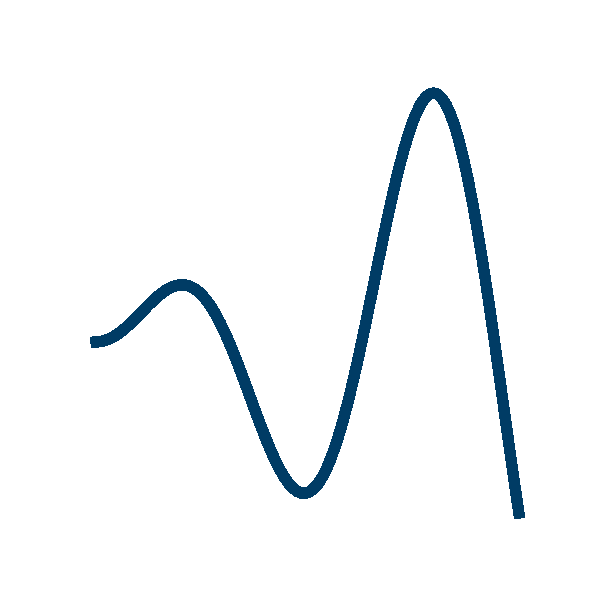
\includegraphics[width=2cm]{time/fig1.pdf}};
                    \node[] at (-5.5,1.5) {Input $x(t)$};
                    \node[] at (8,0)  (TOUT) {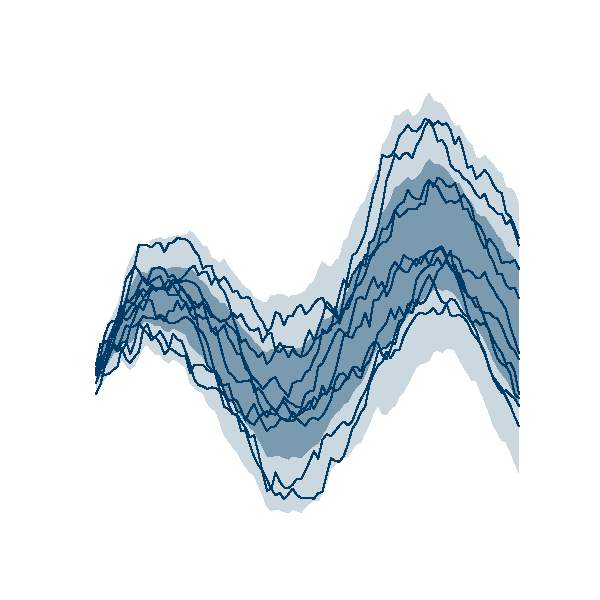
\includegraphics[width=3cm]{time/fig2.pdf}};
                    \node[] at (8,1.5) {Prediction $y(t)$};
                    % Reservoir
                    \node (circle) [draw, circle, minimum size = 2.5cm,inner sep=-5pt, color=green,very thick,text width=2.5cm,align=center] at (0, 0) (RES) {
                        };
                        \node[] at (0,1.5) {Reservoir $u(t)$};
                        \def\mx{-5.2}
                        \def\my{-1.6}
                        \drawqubit{4.6+\mx}{2.2+\my}{.2};
                        \drawqubit{5.2+\mx}{2.2+\my}{.2};
                \drawqubit{5.8+\mx}{2.2+\my}{.2};
                \drawqubit{4.6+\mx}{1.6+\my}{.2};
                \drawqubit{5.2+\mx}{1.6+\my}{.2};
                \drawqubit{5.8+\mx}{1.6+\my}{.2};
                \drawqubit{4.6+\mx}{1.+\my}{.2};
                \drawqubit{5.2+\mx}{1.+\my}{.2};
                \drawqubit{5.8+\mx}{1.+\my}{.2};

                % Arrows
                \draw[-Latex,ultra thick,blue] (IN) -- node [above, blue] {$W_{in}$}(RES);
                \draw[-Latex,ultra thick,blue] (RES) -- node [above, blue] {$W_{out}$}(OUT);
                % \draw[-Latex,ultra thick,green] (RES) -- node [above, green] {$W_{out}$} node [below, green] {optimized}(OUT);
                \draw[-Latex,ultra thick,blue] (TIN) -- (IN);
                \draw[-Latex,ultra thick,blue] (OUT) -- (4,0);
                \draw[-Latex,ultra thick,blue] (6,0) -- (6.75,0);

                \foreach \N [count=\lay,remember={\N as \Nprev (initially 0);}] in {3,2,2}{ % loop over layers
                \foreach \i [evaluate={\y=(\N/2-\i)/2+.25; \x=3.625+\lay/1.5; \prev=int(\lay-1);}] in {1,...,\N}{ % loop over nodes
                \node[thick,draw=blue,fill=blue!20,circle] (N\lay-\i) at (\x,\y) {};
                \ifnum\Nprev>0 % connect to previous layer
                \foreach \j in {1,...,\Nprev}{ % loop over nodes in previous layer
                \draw[thick] (N\prev-\j) -- (N\lay-\i);
                }
                \fi
                }
                }
                \node[] at (5,1.5) {ML};
            \end{tikzpicture}
            % \captionof{figure}{A quantum reservoir system consists of a learning task, an en- and de-coder (red) and the dynamic system itself (green). In standard RC the machine learning part is linear regression.
            % }
\end{document}

